\documentclass[palatino,nosec]{Docencia}


\title{Cuaderno de clase}
\author{Víctor de Juan}
\date{17/18}

\begin{abstract}
Cuaderno de clase de Matemáticas I, con el desarrollo continuado (sin estar separado por sesiones).
\end{abstract}

% Paquetes adicionales

\usepackage[author={Víctor de Juan, 2017}]{pdfcomment}

\makeatletter
\newcommand{\annotate}[2][]{%
\pdfstringdef\x@title{#1}%
\edef\r{\string\r}%
\pdfstringdef\x@contents{#2}%
\pdfannot
width 2\baselineskip
height 2\baselineskip
depth 0pt
{
/Subtype /Text
/T (\x@title)
/Contents (\x@contents)
}%
}
\makeatother

% --------------------
\newcommand{\cimplies}{\text{\hl{$\implies$}}}

\begin{document}
\pagestyle{plain}
\maketitle
\tableofcontents


%% Contenido.

\chapter{Primera evaluación}

\section{Introducción a la asignatura}


Hola, soy Víctor y voy a ser vuestro profesor de matemáticas este año. Algunos me conoceréis, tal vez de campamento o de verme en misa. Para otros tal vez soy totalmente nuevo. ¡Genial! \hl{Soy matemático, entre otras cosas}, y espero poder transmitiros la belleza que encierran las matemáticas.

Reitero que me llamo Víctor y así quiero que me llaméis, ¿bien?

\subsection{Las matemáticas son para siempre}

\href{https://www.ted.com/talks/eduardo_saenz_de_cabezon_math_is_forever}{Vídeo de Eduardo Saenz}

\paragraph{Comentarios al vídeo:}

\begin{itemize}
\item Un teorema es para siempre. ¿Os lo había dicho alguien alguna vez? ¿Qué teoremas conocéis? (Resto, factor, Pitágoras, Tales,  Altura, Euler (V+C=A+2),  ) Pero hay que demostrarlo.
\item Este año está lleno de para siempres. Os voy a enseñar unos buenos teoremas con sus demostraciones a lo largo del curso y vamos a darle importancia a las demostraciones de los contenidos. Cuando la demostración utilice matemáticas que sabéis, las desarrollaremos. 
\subitem \hl{Espero, al final de la clase}, poder enseñaros concretamente a qué me refiero.
\item ¿Alguna pregunta del vídeo? 
\item Weaire-Phelan:
\subitem En la naturaleza, aparece en estructuras químicas (un tipo de cristal).
\subitem \href{https://www.e-architect.co.uk/images/jpgs/beijing/watercube_ptw051208_7.jpg}{El estadio de Pekín de Phelps}
\end{itemize}

\hl{Sed “críticos” en general}. Lo que os cuenten razonadlo. No os lo creáis sin más. Y de esto, nos vamos a hartar en Matemáticas. ¿Alguna pregunta?

\subsubsection{Temario de la asignatura}

El \hl{orden} que vamos a seguir difiere un poco del del libro, porque así nos parece a MariNieves y a mi. 

Vamos a dar un paso más en la resolución de \hl{ecuaciones y sistemas}. 
%
El año pasado resolvíais ecuaciones del tipo: $81^{2x} = \frac{1}{3};\quad x-\sqrt{x-3} = \sqrt{x-2}$, sistemas de ecuaciones 2x2... Este año vamos a ir más allá, vamos a resolver sistemas de 3x3. 

El año pasado tuvisteis una introducción a la geometría. Este año vamos a trabajar con \hl{problemas serios el plano}: distancia punto a recta, distancia entre rectas, cónicas... Por cierto, \ul{¿sabéis porqué se llaman cónicas?}

Y ahora que ya sabéis algo de trigonometría, vamos a ir más allá. Vamos a \hl{exprimir la trigonometría} hasta dominarla. Es algo fundamental en matemáticas. 

Y vamos a dar uno de los temas más bonitos de todo el bachillerato. ¡\hl{Los números complejos}! ¿A alguien le dice algo? ¿A alguien le suena? 
%
Ya veréis que, en realidad, no difíciles. Simplemente arrastramos $\sqrt{-1}$ en las operaciones, como una expresión algebraica, llamando $i=\sqrt{-1}$. 
%
Precioso. 

Y uno de los contenidos centrales del curso, del que hablaréis cuando terminéis el colegio y habréis oído hablar... Las míticas \hl{derivadas}. Os suena, ¿no? 
%
Pues este año nos meteremos en ese berenjenal, a aprender qué es una derivada y para que sirve.
%
También veremos las \hl{Integrales}.
%
Terminaremos el curso con probabilidad y estadística.

Todo esto es una visión general del temario del curso. 
%
Pero hay otro aspecto fundamental de la asignatura. 
%
En otros años lo fundamental puede ser coger habilidad y soltura en los cálculos, saber resolver los problemas... 
%
Este curso va de \hl{razonar y justificar}. Me importa relativamente poco si el resultado está bien o no, en comparación con lo que me importa si el procedimiento está razonado y justificado. 
%
Las matemáticas no son magia, todo tiene una razón de ser. Todo tiene una explicación. 
%
Por ejemplo, ya no nos vamos a centrar tanto en "resuelve esto o lo otro", sino en "demuestra, comprueba, discute esto o lo otro".
%
¿Se entiende?

Por ejemplo, ¿porqué el \hl{teorema de Pitágoras} funciona? 
%
Claro, porque probando con unos números funciona. 
%
¿Quién te asegura que para absolutamente cualquier triángulo rectángulo va a funcionar? Eso hace 4 años te lo creíste. 
%
Este año vamos a demostrar el teorema.

En general, va a haber pocos actos de fe. 
%
En el curso habrá demostraciones y los contenidos no vendrán dados por arte de magia. 
%
Ojo, el teorema fundamental del álgebra no lo podremos demostrar porque hacen falta matemáticas más complejas. 
%
Todo lo demás, lo podremos demostrar.

\subsection{Criterios de evaluación}

Esta asignatura tiene evaluación continua. Eso significa que no hay una recuperación exclusiva para quienes suspendan una evaluación, sino que la primera evaluación es contenido evaluable de la segunda, y la segunda de la tercera.
%
(La primera de la tercera no).

Hay 2 exámenes por evaluación, el primero vale \hl{$\rfrac{1}{3}$} y el segundo \hl{$\rfrac{2}{3}$}. 
%
En ese primer examen, la mitad corresponderá a la evaluación pasada (en caso de que haya evaluación pasada).
%
Si tienes la evaluación suspensa, tienes 5 puntos en el primer examen para recuperar.
%
Si tienes la evaluación aprobada, tienes 5 puntos en el primer examen para repasar.
%
En el segundo examen, en principio, no pondremos contenido de la evaluación anterior.


\section{Números reales}

\subsection{Introducción}

\subsubsection{Conjuntos numéricos}

¿Qué conjuntos de números conocéis? $ℕ,ℤ,ℚ,I,ℝ,ℂ$ \hl{Diagrama de contenidos}.

Cómo distinguir que un número dado pertenece a un conjunto o no.
%
Por ejemplo, $\sqrt{2}$. ¿A qué conjunto pertenece y porqué?
%
\hl{¿Por qué $\sqrt{2}$ es irracional?} $\rfrac{4}{3} = 1.\hat{3}$ también tiene infinitos decimales.
%
En este curso ya no vale creerse lo que los profesores os contamos sin más. Es fundamental entender las demostraciones y ser capaz de razonar el porqué de los asuntos.


\begin{proof}[\textbf{Reducción al absurdo}]
Suponemos $\sqrt{2}\in ℚ$.

Entonces 
\[
	\exists a,b\inℤ \tq \left(\sqrt{2} = \rfrac{a}{b}\right) \wedge \left( \mcd{a,b} = 1 \right)
\]


\[
	\sqrt{2} = \frac{a}{b} \implies 2·b^2 = a^2 \implies a^2 \text{ es par} \overset{1}{\implies} a \text{ es par}
\]

Si $a^2$ es par, necesariamente $a$ es par también. Por reducción al absurdo, si $a$ no fuera par, $a·a$, producto de impares no sería par. 
%
Como $a$ es par, podemos escribirlo como $a=2·k$, para algún $k\in ℤ$. 

\[
	2b^2 = (2k)^2 \implies b^2 = 2k^2 \overset{1}{\implies} b \text{ par}.
\]

Conclusión: $\mcd{a,b} = 2 ≠ 1$. Hemos llegado a una contradicción partiendo de un supuesto ($\sqrt{2}\in ℚ$) "inventado", por lo que ese supuesto debe ser falso. 
\end{proof}

\paragraph{\hl{No os creáis cualquier demostración:}}
Partiendo de $x=y$

\[
x^2 = xy \dimplies x^2-y^2 = xy-y^2 \dimplies (x+y)(x-y) = y(x-y) \dimplies x+y = y \dimplies 2y = y \implies \text{\hl{2=1}}
\]

\nota{Si sobrara tiempo: belleza intrínseca de las matemáticas: ¿Qué hay más, enteros o pares?}


\todo{Sesión 1}

\subsubsection{Grupo y Cuerpo}

\begin{defn}[Grupo]
Sea un conjunto $G\neq \emptyset$ y $\ast$ una operación (ley de composición interna), diremos que $(G,\ast)$ es un grupo si cumple las siguientes propiedades:
\begin{enumerate}
	\item \textbf{Cerrado por la operación}. $\forall x, y \in G, \; x \ast y \in G$
	\item \textbf{Asociatividad}. $\forall x, y, z \in G, \; (x \ast y) \ast z = x \ast (y \ast z)$
	\item \textbf{Existencia del elemento neutro}. $\exists  e \in G \tq ,\; \forall\, x\in G\; x\ast e=x$.
	\item \textbf{Existencia del inverso}. $\forall x \in G ,\; \exists x' \in G \tq x\ast x'=x'\ast x=e$.
\end{enumerate}
\end{defn}

\begin{prop}[Unicidad\IS del neutro e inverso]
  En todo grupo se cumplen las propiedades de unicidad del elemento neutro y del inverso.
\end{prop}

\begin{proof}[\textbf{Reducción al absurdo}]
Primero demostramos que el neutro es único. \\
Sean $e$, y $e'$ dos elementos neutros de $G$, se cumple que $e\ast e'\overset{1}{=}e'$, pero también se cumple que $e'\ast e\overset{2}{=}e$. Esto implica que $e'=e$.\\
1: $e$ elemento neutro.\\
2: $e'$ elemento neutro.

Por otro lado, si suponemos la existencia de dos elementos inversos $a',a''\in G$, entonces $e=a\ast a'=a\ast a''$. \\

\[
	aa' = aa'' \dimplies a'(aa') = a'(aa'') \overset{asoc.}{\dimplies} (a'a)a'=(a'a)a'' \overset{e.n.}{\dimplies} a'=a'' 
\]
\end{proof}

\begin{example}
	\begin{itemize}
		\item Sí: $(ℤ,+),(ℚ,+),(ℝ,+),(\{0,1\},+)$
		\item No: $(ℕ,+),(ℤ,·),(?,·)$
		\item No: $(I,+)$ porque $(1+\sqrt{2}) - (\sqrt{2}\in ℤ)$
	\end{itemize}
\end{example}

\nota{Si el grupo es \hl{conmutativo}, se llama grupo conmutativo o abeliano por el matemático noruego Abel del siglo XIX.}

El \hl{producto tiene problemas} para ser ley de composición interna de grupos. 
%
Sin embargo, podemos considerar $(ℚ,+,·)$. 
%
Ahora hay 2 operaciones y por lo tanto no podemos considerarlo grupo.


\begin{defn}[Cuerpo] 
Sea $K$ un conjunto y sean $(+)$ y $(·)$ dos operaciones binarias cerradas, llamadas suma y producto. 
%
$(K,+,·)$ es un cuerpo si se cumple:
\begin{enumerate}
\item $(A, +)$ es un grupo abeliano.
\item El producto es asociativo.
\item Se cumplen las leyes distributivas: 
	\subitem $\forall a,b,c \in A \; a\cdot(b+c)=a\cdot b + a\cdot c$ 
	\subitem $(a+b)\cdot c= a \cdot c + b \cdot c$
\item El producto es conmutativo.
\item Existe elemento neutro para el producto.
\item $\left(A\backslash \{0\},·\right)$ es un grupo. (Siendo 0 el elemento neutro de la suma.)
\end{enumerate}
\end{defn}

\nota{Si sólo se cumplen a,b,c se llama anillo.}

\begin{example}
	\begin{itemize}
		\item Sí: $(ℝ,+,·),(ℚ,+,·),\left[(ℂ,+,·)\right]$
		\item No: $(ℤ,+,·),\left[(\mathcal{M},+,·)\right]$
		\item $\left(I,+,·\right)$ no, porque $(I,+)$ no es un grupo.
	\end{itemize}
\end{example}


\subsubsection{Entornos (libro):} Dado un intervalo $(3,7)$, ¿cuál es su centro? ¿cuál es su amplitud? (Calcular). A veces nos interesará escribir el mismo intervalo de puntos haciendo énfasis en el centro y el radio. 
%
Entonces, estaremos escribiendo \textit{entornos} en lugar de intervalos. 
%
Y como los intervalos, hay varios tipos de entornos.

\begin{defn}[Entorno\IS abierto]
Llamamos entorno abierto de centro $a$ y radio $r$, y se denota por $E_r(a)$, al conjunto de puntos que distan de $a$ a una distancia menor que $r$:

\[
	E_r(a) = \{x\in\real, |x-a| < r\} = (a-r, a+r) 
\]
\end{defn}

\begin{defn}[Entorno\IS cerrado]
Llamamos entorno cerrado de centro $a$ y radio $r$, y se denota por $E_r(a)$, al conjunto de puntos que distan de $a$ a una distancia menor o igual que $r$::
\[
	E_r[a]  = \{x\in\real, |x-a| \leq r\} = [a-r, a+r]
\]
\end{defn}

\begin{defn}[Entorno\IS reducido]
Llamamos entorno reducido de centro $a$ y radio $r$, y se denota por $E_r(a)$ a:
\[
	E^{\ast}_r(a) = \{x\in\real, |x-a| < r\} - \{a\} = (a-r,a) \cup (a, a+r)
\]
\end{defn}

\nota{El libro utiliza otra notación que no nos gusta. Apuntad la buena.}

\hl{Seguimos pasando páginas del libro y comentando}

\subsection{Logaritmos}

\paragraph{\annotate{En la sesión vimos el vídeo. Como 10-12 se enteraron más o menos bien. 2 no se enteraron de absolutamente nada. Creo que mejor no ponerlo años sucesivos.}{Introducción}}

Vamos a aprender una nueva manera de multiplicar. En realidad ya sabéis, aunque no seáis conscientes.\footnote{Fuente: \href{https://www.youtube.com/watch?v=FB3\_BeukBBk\&t=99s}{Mark Foskey, youtube.com}}





\begin{itemize}
\item Caso 1: $1000000·10000000 = 10^6·10^7 = 10^{13}$. ¿Y podremos hacer esto con otros números que no sean el 10?

\item Caso 2: $64·128 = 2^6·2^7 = 2^{13} = 8192$
\item ¿Caso 3?: Me construyo la tabla del 3.
\begin{center}
\begin{tabular}{cccccccccccc}
1& 3& 9& 27& 81& 243& 729& 2187& 6561& 19683& 59049& 177147\\
\textcolor{red}{0} & \textcolor{red}{1} & \textcolor{red}{2} & \textcolor{red}{3} & \textcolor{red}{4} & \textcolor{red}{5} & \textcolor{red}{6} & \textcolor{red}{7} & \textcolor{red}{8} & \textcolor{red}{9} & \textcolor{red}{10} & \textcolor{red}{11}
\end{tabular}
\end{center}
\item Caso 4: ¿Y para números que no son potencias enteras? Por ejemplo, $64*40$. Pues si $32=2^5$ y $64=2^6$, $40=2^{5,...}$ ¿Tiene sentido?
\item Caso 5: Lo que hicieron, Yost y Napier, fue coger la tabla del 1,0001 en lugar de la tabla del 3 y dividir por mil los números rojos, dando lugar a la tabla de logaritmos:

\begin{center}
	\begin{tabular}{cl}
		0.0 & 1.0\\
		0.001 & 1.001\\
		0.002 & 1.002\\
		0.003 & 1.003\\
		0.004 & 1.00401\\
		0.005 & 1.00501\\
		0.006 & 1.00602\\
		0.007 & 1.00702\\
		0.008 & 1.00803\\
		0.009 & 1.00904\\
		$\vdots$ & \quad\quad$\vdots$\\
		0.991 & 2.69259\\
		0.992 & 2.69529\\
		0.993 & 2.69798\\
		0.994 & 2.70068\\
		0.995 & 2.70338\\
		0.996 & 2.70608\\
		0.997 & 2.70879\\
		0.998 & 2.7115\\
		0.999 & 2.71421\\
		1.0 & \hl{2.71692} (Una aproximación de $e$)\\
	\end{tabular}
\end{center}

\end{itemize}

\begin{defn}[Logaritmo]
Sean $a\in ℝ>0,a≠1$ y $N\in\real$.

Se llama logaritmo en base $a$ de $N$ al exponente $x$ que cumple: $a^x = N$ y se escribe:
\[
	\log_aN=x\dimplies a^x=N
\]
\end{defn}

\nota{De la propia definición se entiende:}
\begin{enumerate}
	\item $y\in\real, y<0 \implies ∀a,\nexists\log_a y$
	\item $\log_a 1 = 0 \dimplies a^0 = 1$
	\item $\log_a a = 1 \dimplies a^1 = a$
	\item $\log_a a^q = q \dimplies a^q = a^q$ por definición.
	\item $a^{\log_a N} = N$
\todo{Sesión 2}
	\begin{proof}
		Sea $b = \log_a N \dimplies a^b = N$.

		Entonces, $a^{\log_a N} = N \dimplies a^n = N$
	\end{proof}
\end{enumerate}



\paragraph{Propiedades:}
\begin{itemize}
	\item $\log_a(AB) = \log_a(A) + \log_a(B)$
		\begin{proof}
			\[\left.\begin{array}{c}
				\log_a(A) = p \dimplies a^p = A\\
				\log_a(B) = p \dimplies a^q = B
			\end{array}\right\}\implies A·B = a^{p+q} \implies \log_a(AB) = \log_aa^{p+q}\]
			\[
				\log_a(AB) = \log_aa^{p+q} \overset{?}{\implies} \log_a(AB) = p+q \overset{?}{=} \log_aA + \log_aB
			\]
		\end{proof}
	\item $\log_a\left(\rfrac{A}{B}\right) = \log_a(A) - \log_a(B)$
	\begin{proof}
		Análoga. Para completar por vosotros. Si no lo conseguís, intentadlo.
	\end{proof}
	\item $\log_a(A)^n = n·\log_a(A)$ \hl{\textbf{Ojo:} $\left[\log_a(A+B)\right]^n \neq n·\log_a(A)$}
	\begin{proof}
		Tomamos $\log_aA = p \dimplies a^p = A$

		\[
			a^p = A \dimplies a^{np}=A^n \dimplies \log_aa^{np} = \log_aA^n \dimplies np = \log_aA^n
		\]
		\[ 
			\dimplies n\log_aA = \log_aA^n
		\]
	\end{proof}
	\item $\displaystyle\log_aA = \frac{\log_bA}{\log_ba}$ \textbf{(Cambio de base})
		\begin{proof}
			Tomamos $\log_aA = p \dimplies a^p = A$
			\[
				\log_ba^p = \log_bA \dimplies p\log_ba = \log_bA \dimplies p=\log_aA=\frac{\log_bA}{\log_ba}
			\]

		\end{proof}
\end{itemize}

\paragraph{Tomar logaritmos:}

\[
A = B \overset{1}{\dimplies} a^{\log_a A} = a^{\log_a B} \dimplies \log_aA=\log_aB
\]

\subsubsection{Ejemplos con logaritmos}

\begin{itemize}
	\item $\log \sqrt{0,0001}$
	\item \annotate{Dejé la demostración para que lo hicieran ellos. Se atascaron bastante. No repetir.}{Demuestra} $\log_a b · \log_b a = 1$ 
\end{itemize}

\subsubsection{Ejercicios con logaritmos}
\todo{Sesión 3. Corregimos el 50a, de deberes lo demás para empezar corrigiendo.}
Pág 21, ejers 50,52.

\subsubsection{Aplicación de los logaritmos}

\paragraph{pH}

Para medir el nivel de acidez, pH, que mide la concentración de iones hidronio ($H_3O^+$)

\[pH=-\log[H_30^+]\]

\paragraph*{Despejar el tiempo} En el crecimiento exponencial de bacterias:
$P = p_0·k^t$ donde $p_0$ es la cantidad inicial, $t$ son los periodos de tiempo y $k$ la tasa de multiplicación.

Pag 23, ejer 57.

\paragraph{Interés compuesto}

\nota{\hl{Que no copien todo esto, sino que lo entiendan.}}

Sea $C$ el capital inicial. Tras 1 periodo de tiempo, obtengo el r\% de intereses. Entonces tendré: $C_1 = C_0 + \rfrac{r}{100}C_0 = C_0·\left(1+\frac{r}{100}\right)$

Pasado otro periodo de tiempo tendré $C_2 = C_1·\left(1+\frac{r}{100}\right) = C_0·\left(1+\frac{r}{100}\right)·\left(1+\frac{r}{100}\right) = C_0 ·\left(1+\frac{r}{100}\right)^2$

En general, para $t$ periodos de tiempo tendremos: $C_t = C_0·\left(1+\frac{r}{100}\right)^t$.

La fórmula del interés compuesto capitalizado en $p$ periodos, \hl{para un interés nominal $r$ es}: 

\[C = C_0·\left(1+\frac{r}{100p}\right)^{pt}\]


\paragraph{3 preguntas? \hl{No.}}
\begin{itemize}
	\item[a] Pero... ¿es lo mismo un interés anual del 5\% capitalizado cada mes, que un interés anual del 5\% capitalizado cada año?

	\item[b] ¿Y si capitalizo cada semana? ¿Y cada día? ¿Y si capitalizo \textit{instantáneamente}? \hl{(Sí)}

	\item[c] ¿Cuánto tiempo tengo que dejar el dinero si quiero ganar una cantidad concreta?
\end{itemize}

\paragraph{a)}
Pero, ¿es lo mismo un interés mensual del 5\% durante 12 meses que un interés anual del 5\% durante 12 meses? Sí. ¿A quién le importa que sean meses o años?

Pero... ¿es lo mismo un interés anual del 5\% capitalizado cada mes, que un interés anual del 5\% capitalizado cada año? ¿Hay alguno que sea mayor? 

\begin{example}

Tengo $C= 1000$ a un $r=5\%$. Tengo 2 opciones para elegir y no se cual es mejor. 

\begin{itemize}
	\item[a)] Un interés anual del 5\% capitalizado cada mes durante 5 años.

	\[
		C = C_0·(1+\rfrac{r}{100p})^{t·p} = 1000·(1+\rfrac{5}{1200})^{12*5} = 1283.36
	\]
	\item[b)] Un interés anual del 5\% capitalizado cada año durante 5 años.

	\[
		C = C_0·(1+\rfrac{r}{100p})^{t·p} = 1000·(1+\rfrac{5}{100})^{5} = 1276.28
	\]

	Es más rentable la opción a. 

	\nota{\hl{De hecho}, ¿cuál es el interés equivalente que hay que aplicar al año en el caso a)?}

	\[
		C = C_0·(1+\rfrac{r}{100})^{t} \dimplies \frac{C}{C_0} = (1+\rfrac{r}{100})^t \implies \sqrt[t]{\frac{C}{C_0}} = \sqrt[t]{(1+\rfrac{r}{100})^t} \dimplies
	\]
	\[
 		\sqrt[t]{\frac{C}{C_0}} -1 = \rfrac{r}{100} \dimplies r = 100·\left(\sqrt[t]{\frac{C}{C_0}} -1 \right)\implies r = 100·\left(\sqrt[5]{\frac{1283.36}{1000}} - 1\right) = 5.1162...
	\]

	Conclusión, un 5\% mensual es lo mismo que un 5.1162...\% anual. Por esto, y para que no nos puedan timar los bancos existe la \concept{TAE} (Tasa Anual Equivalente.)


\end{itemize}
\end{example}

\paragraph{b)}
¿Y si capitalizo cada semana? ¿Y cada día? ¿Y si capitalizo \textit{instantáneamente}? 

\paragraph{c)}
Tengo entendido que durante el mes de julio, Miguel ha trabajado de hamaquero en la playa y cobrado 150 al mes. ¿Puede ser? Su banco le ofrece un depósito con un interés del 10\% y Miguel querría pagarse su carrera, que será algo así como 10000, sino sigue subiendo.
%
¿Cuánto tiempo tiene que dejar su dinero en el banco para pagarse la carrera?

\[
	C = C_0·(1+\rfrac{r}{100})^{t} \dimplies \log\frac{C}{C_0} = t\log(1+\rfrac{r}{100}) \dimplies t = \frac{\log\frac{C}{C_0}}{\log(1+\rfrac{r}{100})} = \frac{\log\frac{10000}{150}}{\log\left(1+\rfrac{10}{100}\right)} 
\]

\[
	t = 44.06\text{ años}
\]

De momento lo dejamos aquí. El próximo tema que tiene ecuaciones volveremos a trabajar con el interés, las bacterias, etc.

\todo{Fin sesión 4.}

\section{Tema 2: álgebra}

\subsection{Binomio de Newton}

\paragraph{Combinatoria básica} ¿Cuántas parejas puedo hacer con 5 cartas? $\binom{5}{2}$

\begin{defn}[Número combinatorio] Dados 2 números naturales no nulos $m$ y $n$, siendo $m≥n$, se denomina número combinatorio $\binom{m}{n}$, y se lee "m" sobre "n" a $\binom{m}{n} = \frac{m!}{n!(m-n)!}$
\end{defn}

\paragraph{Propiedades}
\begin{itemize}
	\item $\binom{m}{0}=\binom{m}{m}=1$
	\begin{proof}
		\[\binom{m}{m} = \frac{m!}{m!(m-m)!} = 1\]
	\end{proof}
	\item $\binom{m}{n}=\binom{m}{m-n}$ 
	\begin{proof}
		\[\binom{m}{n} = \frac{m!}{n!(m-n)!} = \frac{m!}{(m-(m-n))!(m-n)!} = \binom{m}{m-n} \]
	\end{proof}
	\item $\binom{m}{n} + \binom{m}{n+1}=\binom{m+1}{n+1}$
	\begin{proof}
		\[
			\binom{m}{n} + \binom{m}{n+1} = \frac{m!}{n!(m-n)!} + \frac{m!}{(n+1)!(m-n-1)!} = 
		\]
		\[
			\frac{m!(n+1)}{(n+1)n!(m-n)!} + \frac{m!(m-n)}{(n+1)!(m-n-1)!(m-n)}
		\]
		\[
			\frac{m!(n+1+m-n)}{(n+1)!(m-n)!} = \frac{(m+1)!}{(n+1)!(m-n)!} = 
		\frac{(m+1)!}{(n+1)!((m+1)-(n+1))!} = \binom{m+1}{n+1}
		\]
	\end{proof}
\end{itemize}

\nota{No copiar}

En cursos anteriores hemos visto $(a+b)^2 = a^2+2ab+b^2$. Si tenemos muy buena memoria igual recordamos $(a+b)^3 = a^3+3ab^2+3a^2b+a^3$. Pero, ¿cómo calcular, sin desarrollar $(a+b)^6$? 

$(a+b)^6 = (a+b)(a+b)(a+b)(a+b)(a+b)(a+b)(a+b)$ ¿Cuántos productos $abbbbb$ va a haber? $babbbb,bbabbb,bbbabb,bbbbab,bbbbba$. Esto es lo mismo que preguntarnos, ¿de cuántas maneras diferentes puedo ordenar la secuencia de letras $abbbbb$? O, lo que es lo mismo, ¿cuántas combinaciones hay de colocar la $a$ en las 6 posiciones?
%
¿Y para el producto $aabbbb$? Hay 6 huecos y queremos rellenar 2 de ellos con $a$ y dejar 4 libres (fijémonos que es lo mismo que querer rellenar 4 con $b$ y dejar 2 libres. Debemos obtener las mismas posibilidades). ¿De cuántas maneras lo puedo hacer? ¿Cuántas parejas de casilleros puedo hacer con 6 casilleros?

Razonando de esta manera, llegamos a que el coeficiente de $aabbbb = a^2b^4 = \binom{6}{2}=\binom{6}{4}$. Repitiendo el razonamiento, llegaríamos a que el coeficiente sería $a^{m-n}b^m = \binom{m}{n}$. 

De esta manera podemos escribir:

\[
	(a+b)^6 = \binom{6}{0}a^0b^6 + \binom{6}{1}a^1b^5 + \binom{6}{2}a^2b^4 + ... = \sum_{i=0}^6 \binom{6}{i}a^ib^{6-i}
\]

Generalizando esta idea para cualquier exponente $n$ obtenemos:

\concept{Binomio de Newton}:
$
\displaystyle (a\text{\hl{+}}b)^n = \sum_{i=0}^n \binom{n}{i} a^ib^{n-i}
$

\paragraph{Curiosidad matemática:} Triángulo de Pascal.

De aquí construimos el triángulo y jugamos un rato con él. Potencias de 2 sumando los números, potencias de 11 y Fibonnaci.

\begin{figure}[hbpt]
	\centering
	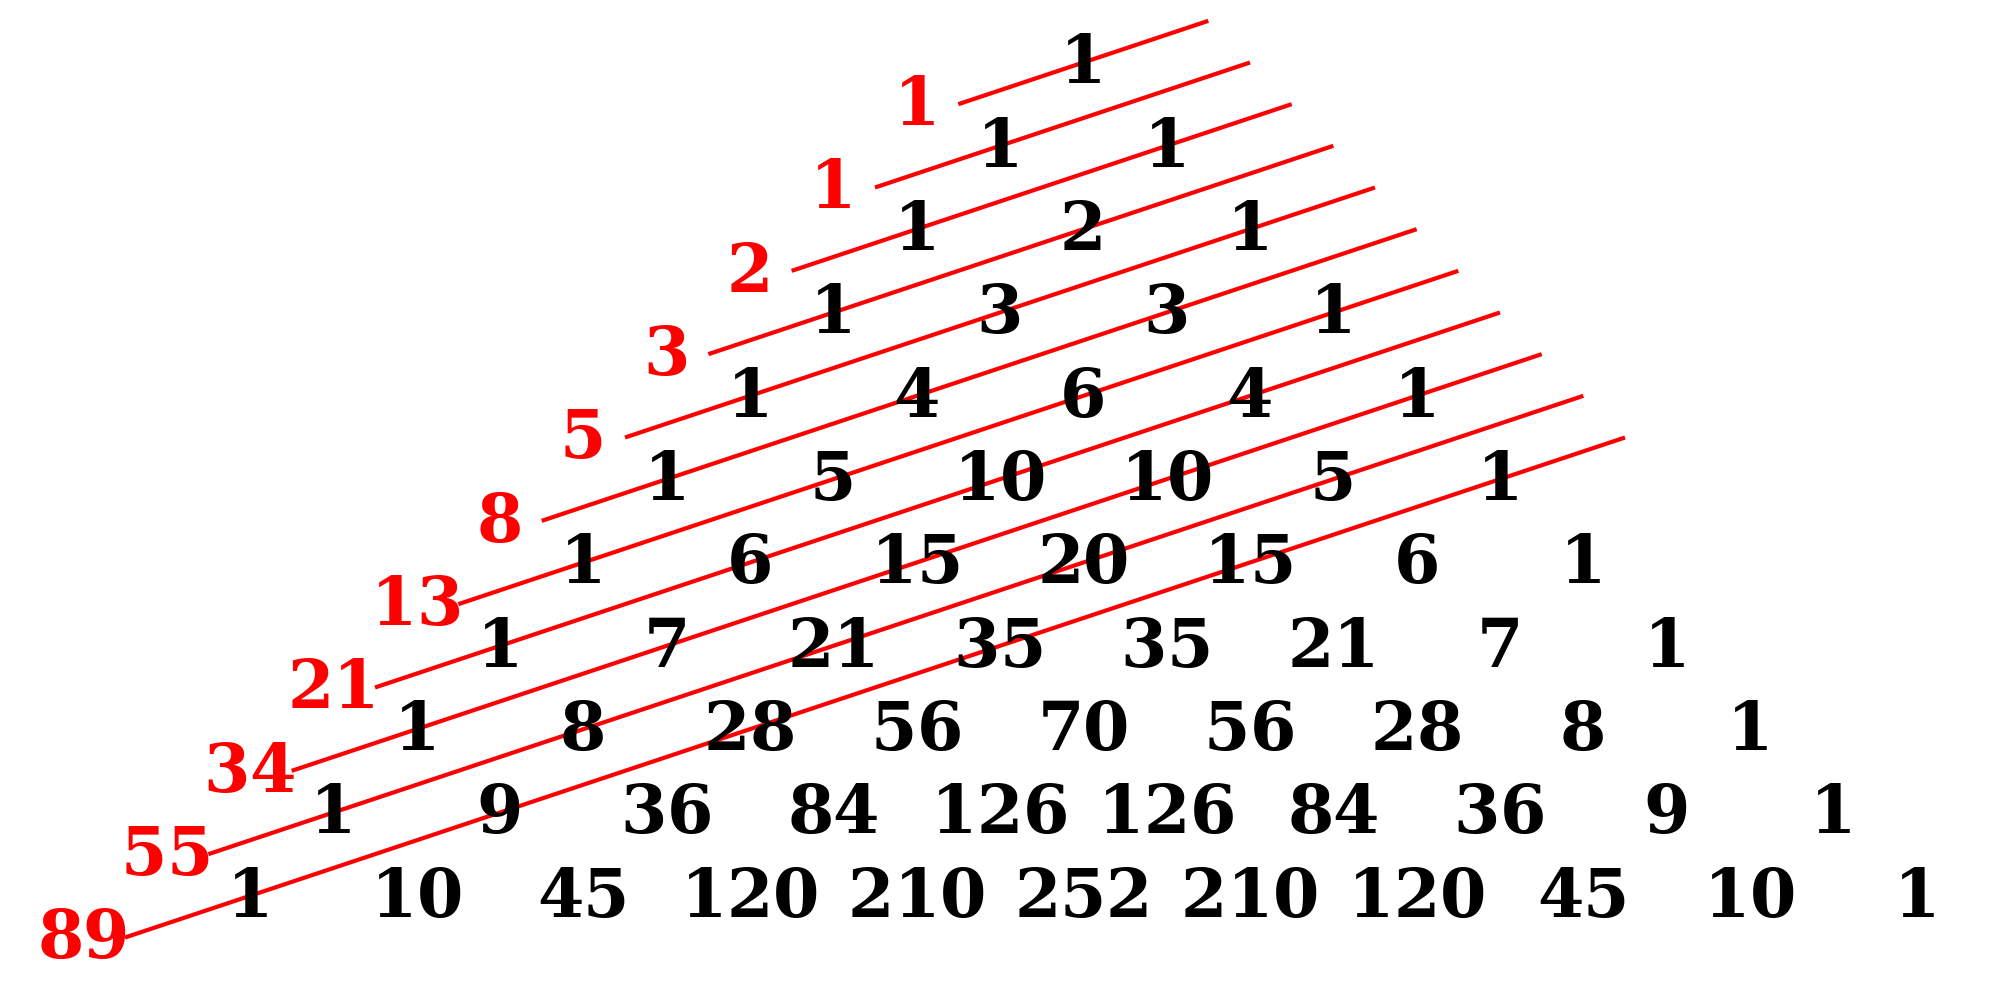
\includegraphics[scale=0.17]{img/Pascal.png}
	\label{img::TrianguloPascal}
	\caption{Triángulo de Pascal y su relación con la serie de Fibonacci}
\end{figure}


\todo{Fin sesión. Demasiado tiempo invertido en esto para lo que en realidad es.}
Triángulo de Pascal (vídeo brutal de \href{https://www.youtube.com/watch?v=0iMtlus-afo}{Numberphile})

\paragraph{\hl{Sesión 21/09}:} Empezar con un ejemplo de uso de la fórmula para $(3x-2)^5$. Así, utilizamos la calculadora para números combinatorios. 
Ejercicios del libro. (Yo 15, 16. Ellos 20 y 21).


\subsection{Teoremas de factorización}

\paragraph{Sesión 22/09:} Empezar con título. 2.2) Factorización. Ejemplo. La factorización del polinomio. ¿Qué raíces puede tener? Ni $\pm1,\pm3$, ¿entonces? Teorema de las raíces racionales.

Factoriza (yo con ellos): $P(x) = 3x^3-x^2+9x-3 = 3(x^2+3)\left(x-\rfrac{1}{3}\right)$

\begin{theorem}[Teorema\IS del factor]
Sea $P(x) = a_nx^n+a_{n-1}x^{n-1}+...+a_1x+a_0$ con $a_n≠0$ y $a_n,a_{n-1},...,a_1,a_0\in\real$. 
Sea $α\in\real$.

\[
	P(α) = 0 \dimplies \frac{P(x)}{(x-α)} = Q(x)
\]
\end{theorem}

De hecho este teorema es un caso particular del teorema del resto:
\begin{theorem}[Teorema\IS del resto]
Sea $P(x) = a_nx^n+a_{n-1}x^{n-1}+...+a_1x+a_0$ con $a_n≠0$ y $a_n,a_{n-1},...,a_1,a_0\in\real$.

Entonces, el resto de $\frac{P(x)}{x-α} = P(α)$
\end{theorem}


\begin{theorem}[Teorema\IS de la factorización]
Sea $P(x) = a_nx^n+a_{n-1}x^{n-1}+...+a_1x+a_0$ con $a_n≠0$ y $a_n,a_{n-1},...,a_1,a_0\in\real$ y $α_1,α_2,...,α_n\in\real$ las raíces o ceros de $P(x)$. 

Entonces,\[P(x) = a_n(x-α_1)(x-α_2)...(x-α_n)\]
\end{theorem}


\begin{theorem}[Teorema\IS de las raíces enteras]
Sea $P(x) = a_nx^n+a_{n-1}x^{n-1}+...+a_1x+a_0$, con $a_n≠0$, una raíz entera $r$ de $P(x)$ tiene que ser divisor del término independiente.
\end{theorem}



\begin{theorem}[Teorema\IS de las raíces racionales]
Sea $P(x) = a_nx^n+a_{n-1}x^{n-1}+...+a_1x+a_0$, con $a_n≠0$,$a_i\inℤ$ una raíz fraccionaria $\rfrac{n}{m}$ del polinomio $P(x)$ tiene que cumplir $n|a_0$ y $m|a_n$.
\end{theorem}


\subsubsection{Ejercicios:}

\begin{enumerate}
\item (YO) Sea $P(x) = 3x^3-3x^2-3x+3 = 3(x-1)(x+1)^2$
\begin{itemize}
	\item ¿Es divisible por $(x-1)$? Comprobamos $P(1) = 3-3-3+3 = 0 \overset{T.F}{\implies}$ Sí.
\end{itemize}

\item (YO) Sea $P(x) = 6x^3-10x^2+4x = 6x(x-1)(x-\rfrac{2}{3})$ 
\begin{itemize}
	\item Factoriza.
	\subitem $P(0) = 0$. Por el teorema del factor sabemos que $x-0$ es un factor.
	\subitem Posibles raíces: $n=\pm1,\pm2,\pm4$ y $m=\pm1,\pm2,\pm3,\pm6$	
	\subitem Por el teorema de la factorización, $Q(x) = 3x^3-5x+2x$ tendrá las mismas raíces que $P(x) = 6x^3-10x^2+4x$. \hl{(Ojo, no podemos simplificar, pero las raíces son las mismas)}. Ahora las posibles raíces son $\rfrac{n}{m}$ donde $n\in\{\pm1,\pm2\}$ y $m\in\{\pm1,\pm3\}$
	\subitem $P(1) = 0$. Por el teorema del factor sabemos que $0$ es una raíz. ¿Es esto más fácil que Ruffini? ¿Y ahora?
\end{itemize}

Por grupos los demás ejercicios:
\item Sea $P(x) = 2x^3-2x^2+kx+4$.
\begin{itemize}
	\item Halla el valor de $k$ para que $P(x)$ sea divisible por $x-2$.
	\subitem Por el teorema del factor, buscamos $P(2) = 0$. Entonces:
	\[
		P(2) = 0 \dimplies 2^4-2^3+2k+4 = 0 \dimplies 16-12+2k = 0 \dimplies k = -2
	\]
\end{itemize}


\item Sea $P(x) = x^4+4x^3+6x^2+4x+1$
\begin{itemize}
	\item Factoriza (Newton)
\end{itemize}

\todo{Sesión.}
\paragraph{Sesión 26/09}: \hl{Empezar corrigiendo}.

\item Sea $P(x) = x^3+2·k·x^2+4·k·x+8$
\begin{itemize}
	\item ¿Qué valor puede tomar $k$ para que el polinomio tenga una raíz de multiplicidad 3? (Newton)
\end{itemize}


\item Sea $P(x) = 4x^2+kx+1$.
\begin{itemize}
	\item Halla el valor de $k$ para que sea divisible por $\left(x-\rfrac{1}{3}\right)$. $k=\frac{13}{3}$.
	\item Pero, $3$ no divide a $4$. ¿Cómo podría ser una raíz $\rfrac{1}{3}$?
\end{itemize}


\item Sea $P(x) = 6x^3+ax^2+bx-1$, con $a,b\inℤ$
\begin{itemize}
	\item Halla el valor de $a,b$ para que $P(x)$ sea divisible por $(x-\rfrac{1}{3})$ y por $(x-\rfrac{1}{5})$.
	\subitem Por el teorema de las raíces racionales, $5$ no divide al coeficiente principal, por lo que $P(x)$ no puede ser divisible por $(x-\rfrac{1}{5})$.
	\item Halla el valor de $a,b$ para que $P(x)$ sea divisible por $(x-\rfrac{1}{3})$ y por $(x-\rfrac{1}{2})$.
	\subitem Por el teorema del factor, buscamos:
	\[
	\left\{
		\begin{array}{c}
			P(\rfrac{1}{2}) = 0 \dimplies \frac{6}{8} + \frac{a}{4} + \frac{b}{2} - 1 = 0\\
			P(\rfrac{1}{3}) = 0 \dimplies \frac{6}{27} + \frac{a}{9} + \frac{b}{3} - 1 = 0
		\end{array}\right\}\dimplies ... \quad (a,b) = (-1,-4)
	\]
\end{itemize}

\item\textbf{Ampliación, puesto pero sin corregir} Sea $P(x) = 4x^2+bx+1$, con $b∈ℤ$. 
\begin{itemize}
	\item Sabemos que sus raíces $α_1,α_2$ son fraccionarias y negativas. ¿Cuáles son? ¿Cuánto vale $b$?
	\subitem Por el teorema de las raíces racionales, $α_1 = \rfrac{n_1}{m_1}$, sabemos que $n_1$ divide a $1$. Análogo para $α_2$.

	Por otro lado, sabemos que $m_2$ divide a 4. Las posibilidades son $2,4$, con lo que $α_1,α_2 \in \{\rfrac{1}{2},\rfrac{1}{4}\}$

	Por el teorema del factor, $P(\rfrac{1}{2}) = 1+b\rfrac{1}{2}+1 = 0 \implies b=-4$. 

	Por el teorema del factor, $P(\rfrac{1}{4}) = \rfrac{1}{4}+b\rfrac{1}{4}+1 = 0 \implies b=-2$.

	Si queremos que sea divisible por los 2 factores, b tiene que valer a la vez $4$ y $-2$. Entonces, necesariamente $P(x) = 4(x-\rfrac{1}{2})^2$ o $P(x) = 4(x-\rfrac{1}{4})^2$. 

	Desarrollando la segunda opción, obtenemos como término independiente $\rfrac{1}{4}≠1$, por lo que no es posible. 
	%
	Por otro lado, desarrollando la primera opción obtenemos algo con sentido.

	\[
		4\left(x+\rfrac{1}{2}\right)^2 = 4\left(x^2+x+\rfrac{1}{4}\right) = 4x^2+4x+1 \implies b=4
	\]

\end{itemize}


\item Sea $P(x) = 21x^2+10x-2$. $P(x) + 3 = 21(x+1/3)(x+1/7)$.

\end{enumerate}

\subsection{Ecuaciones}

\subsubsection{Teoría sobre ecuaciones}

\begin{defn}
2 ecuaciones son equivalentes si y solamente si tienen las mismas soluciones.
\end{defn}

\obs Dividir por 0 no mantiene la equivalencia (ver demostración día 1 de $0=1$).

\obs
\[
	-20 = -20 \dimplies 25-45 = 16-36 \dimplies 5^2-5·9 = 4^2-4·9 \dimplies 5^2-5·9+\left(\rfrac{9}{2}\right)^2 = 4^2-4·9+\left(\rfrac{9}{2}\right)^2 \dimplies
\]
\[
	\left(5-\rfrac{9}{2}\right)^2 = \left(4-\rfrac{9}{2}\right)^2 \text{\hl{\;\;;\;\;}} 5-\rfrac{9}{2} = 4-\rfrac{9}{2} \dimplies 5=4
\]
Es decir, en general, tomar una raíz no mantiene equivalencia entre ecuaciones (tampoco elevar a una potencia).

\todo{Sesión}

\paragraph{Sesión 27/09:} 
\begin{itemize}
	\item Empezar preguntando si están todos los ejercicios de polinomios corregidos (Porque yo diría que no). En ese caso, que vayan corrigiendo ellos. 
	%
	Mientras hay algunos en la pizarra, 
\begin{itemize}
	\item Factorizar $P(x) = 9x^3-\frac{27}{2}x^2+\frac{13}{2}x-1 = 9·(x-1/2)(x-2/3)(x-1/3)$. Pista (para ahorraros pruebas innecesarias con Ruffini), todas las raíces son fraccionarias y positivas.

	\item Factorizar $P(x) = x^7+2x^4+x = x(x^3+1)^2$
\end{itemize}
	


	\item 
\end{itemize}

\paragraph{Clasificación de ecuaciones}

Las ecuaciones según sus soluciones pueden ser:
\begin{itemize}
	\item Incompatible: no tiene ninguna solución. Ejemplo: $5x=5x+2$
	\item Compatible determinada: tiene un número finito de soluciones. Ejemplo: $3x=6$.
	\item Compatible indeterminada: tiene infinitas soluciones. Ejemplo $2x-\frac{3x-1}{3} = x+\frac{1}{3}$. Solución: $x=λ, ∀λ∈ℝ$.
\end{itemize}


\subsubsection{Ecuación de segundo grado}

$ax^2+bx+c=0$. ¿Alguien sabe de dónde viene la fórmula?

\[
	x^2+\frac{b}{a}x+\frac{c}{a}=0 \dimplies x^2+2\frac{b}{2a}x+\frac{c}{a}=0\dimplies x^2+2\frac{b}{2a}+\left(\frac{b}{2a}\right)^2-\left(\frac{b}{2a}\right)^2+\frac{c}{a} = 0
\]
\[
	\left(x+\frac{b}{2a}\right)^2 = \frac{b^2}{4a^2}-\frac{c}{a} \implies x+\frac{b}{2a} = \sqrt{\frac{b^2-4ac}{4a^2}} \dimplies x = \frac{\sqrt{b^2-4ac}}{2a} -\frac{b}{2a}
\]

\subsubsection{Racionales}

Ecuaciones racionales.

\paragraph{Ejemplo}
\[
	\frac{2x}{x-2} + \frac{3x}{x+2} = \frac{7x^2}{x^2-4} \dimplies \frac{2x(x+2)}{(x-2)(x+2)} + \frac{3x(x-2)}{(x+2)(x-2)} = \frac{7x^2}{x^2-4} \dimplies 
\]
\[
	\frac{2x(x+2)+3x(x-2)}{x^2-4} = \frac{7x^2}{x^2-4} \text{\hl{$\implies$}} 2x^2+4x+3x^2-6x=7x^2 \dimplies 5x^2-7x^2-2x = 0 \dimplies 
\]
\[
	x(-x-1) = 0 \dimplies x_1 = 0 \wedge x_2 = -1
\]

\hl{¿Son soluciones las 2?}

Para trabajar: Pág 46, ejer 36.

\paragraph{36,a}
\[
	\frac{1}{1-\frac{1}{x+1}} = \frac{x+1}{x} \dimplies \frac{1}{\frac{x+1-1}{x+1}}=\frac{x+1}{x} \dimplies \frac{x+1}{x} = \frac{x+1}{x} \text{\hl{$\implies$}} x+1=x+1 \dimplies x=λ, ∀λ∈ℝ
\]

\paragraph{Sesión 28/09}

\begin{itemize}
	\item Empezar corrigiendo el ejercicio anterior: La solución de la última ecuación sí es $x\inℝ$, pero en la primera, $x\in\{0,-1\}$ no son soluciones.

	\item Definición de ecuación compatible indeterminada.
	
	\item Corregir la otra ecuación (36,b). Mientras alguien la hace en la pizarra, trabajamos con: $2x-\frac{3x-1}{3} = x+\frac{1}{4}$. Solución: ecuación incompatible.
\end{itemize}

\paragraph{36,b}
\[
	\frac{1+\displaystyle\frac{x+1}{x-1}}{2-\displaystyle\frac{x-1}{x+1}}=2 \dimplies \frac{\displaystyle\frac{x-1+x+1}{x-1}}{\displaystyle\frac{2x+2-x+1}{x+1}} = 2 \dimplies
\]
\[	
	\frac{\displaystyle\frac{2x}{x-1}}{\displaystyle\frac{x+3}{x+1}}=2 \dimplies 2x^2+2x=x^2+4x-6 \dimplies 2x=6 \dimplies x=3
\]


Mientras corregimos los 2, para los siguientes \todo{Sin hacer}:

\[
	\frac{3}{x} - \frac{x}{x+2} = \frac{5x-1}{x^2+x-2}
\]

Lo corrigen ellos. El 33.

\subsubsection{Radicales}


\paragraph{Ejemplo:}
\[
	\sqrt{x+1} - \sqrt{x^2-5}=0 \text{\hl{$\implies$}} x+1 = x^2-5 \dimplies (x_0,x_1) = (3,-2)
\]

Comprobamos: $\sqrt{-2+1} = \sqrt{(-2)^2-5} \dimplies \sqrt{-1} = \sqrt{-1}$; -2 no es una solución en los reales.

Por otro lado: $\sqrt{3+1} = \sqrt{3^2-5} \dimplies \sqrt{2}=\sqrt{2}$

\paragraph{Ejercicio:} (creo que está sin corregir)
\[
	\sqrt{x+4}+\sqrt{x-1} = 5 \text{\hl{$\implies$}} (x+4)+(x-1) + 2\sqrt{(x+4)(x-1)} = 25 \text{\hl{$\implies$}} (22-2x)^2 = 4(x^2+3x-4) \dimplies 
\]
\[
	4x^2-88x + 484 = 4x^2+12x-16 \dimplies -100x + 500 = 0 \dimplies x=5
\]

Comprobamos:
\[
	\sqrt{5+4}+\sqrt{5-1} = 3+2 = 5
\]

\paragraph{Ejercicio 40 b:} Truco: aplicar el binomio de Newton.


\paragraph{40 a}

\paragraph{Sesión 29/09}
\begin{itemize}
	\item Empezar con la comprobación del 40 b.
	\item Seguir con la corrección del 40 a, si han tenido problemas.
	\item Empezar logarítmicas.
	\item No preservación de la equivalencia.
	\item Ejemplo de 3 maneras diferentes.
	\item Para trabajar.
	\item Deberes para el martes (salvo que sea el problema los deberes): 
	\[
		\sqrt{x^3+2\sqrt{x^3}+1} = 0 \dimplies \sqrt{(\sqrt{x^3}+1)^2} = 0 \text{\hl{$\implies$}} \sqrt{x^3}=-1 \dimplies x=-1
	\]
	Comprobamos: $\sqrt{(-1)^2+2\sqrt{-1^3}+1} = \sqrt{2+2\sqrt{-1}} \notin ℝ$

	El otro camino:
	\[
		\sqrt{x^3+2\sqrt{x^3}+1} = 0 \implies x^3+2\sqrt{x^3}+1 = 0 \dimplies 2\sqrt{x^3} = -x^3-1 \implies 4x^3=x^6+2x^3+1 \dimplies 
	\]
	\[
		x^6-2x^3+1=0 \dimplies t^2-2t+1=0 \dimplies t_1=-1 \implies x^3=t=-1\implies x=\sqrt[3]{-1}=-1
	\]
	Comprobamos: $\sqrt{(-1)^2+2\sqrt{-1^3}+1} = \sqrt{2+2\sqrt{-1}} \notin ℝ$

\end{itemize}

\subsubsection{Logarítmicas}

Los logaritmos tampoco conservan las equivalencias:

Versión innecesariamente larga:
\[
	-5 = -5 \dimplies -30+25 = 1-6 \dimplies -30+25+9 = 9+1-6 \dimplies (3-5)^2 = (3-1)^2 \dimplies 
\]
\[
	\log(3-5)^2 = \log(3-1)^2 \dimplies 2\log(3-5) = 2\log(3-1) \dimplies \log(3-5)=\log(3-1) \dimplies \log2=\log-2
\]

Versión corta:
\[
	(-2)^2 = (2)^2 \text{\hl{$\implies$}} 2\log(-2) = 2\log(2) \dimplies \log(-2)^2 = \log(2^2) \dimplies \log(-2) = \log(2) \dimplies -2=2
\]

Ecuación de ejemplo:

\[
	5\log x=3\log x+2\log 6 \dimplies 2\log x=2\log6 \text{\hl{$\implies$}} x=6
\]


El libro lo hace de otra manera:

\[
	5\log x=3\log x+2\log 6 \dimplies \log x^5=\log36x^3 \dimplies x^5=36x^3 \dimplies
\]
\[
	x^5-36x^3 = 0 \dimplies x^3(x^2-36) = 0 \dimplies x^3(x+6)(x-6) = 0
\]

Incluso, habría una tercera manera:

\[
	\log x=t \implies 5t=3t+\log6^2 \dimplies 2t=2\log6 \dimplies t=\log6 \dimplies \log x=\log6 \text{\hl{$\implies$}} x=6
\]

Trabajamos: página 48, ejercicio 45 b,d.

\paragraph{45b}
\[
	\log\frac{2x-2}{x} = 2\log(x-1)-\log x \dimplies \log \frac{2x-2}{x}=\log\frac{(x-1)^2}{x} \cimplies \frac{2(x-1)}{x} = \frac{(x-1)^2}{x} \overset{1}{\cimplies}
	\]
	\[ 
	x-1=2 \dimplies x=3
\]
En 1 hemos simplificado 2 factores. $x$ y $(x-1)$. En esta simplificación podríamos haber perdido soluciones, en concreto, si $0,1$ fueran soluciones no lo obtendríamos. 

En este caso no son solución porque $\log 0$ no existe.

\paragraph{45d}
\[
\frac{\log (4-x)}{\log(x+2)}=2 \cimplies \log(4-x) = \log(x+2)^2 \cimplies 4-x=(x+2)^2 \dimplies 4-x=x^2+4x+4 \dimplies
	\]
	\[ x^2+5x=0 \dimplies x_1=0 \wedge x_2=-5
\]
$x_2=-5$ no es solución porque $\nexists\log(-5+2)=\log(-3)$. Por otro lado, $\frac{\log4}{\log2} = \log_24=2$ cqc.

\paragraph{Sesión 3/10}
\begin{itemize}
	\item Empezar re-explicando la pérdida de equivalencias. Cuando simplificamos, marcamos en la equivalencia $x\neq-1$. Al final, comprobamos si los valores intermedios son soluciones o no.
	\item Corregimos el 45bd.
	\item Mientras, trabajar el 46 b.
	\item Comentario al 46a (cambio de base), 45c (rango inexistente).
	\item Problema.
	\item Equivalencia exponenciales. Trabajamos 52 abc, mientras corrigen el d.
\end{itemize}

\paragraph{46a} mientras corrigen

\[
	\log_x 3 = \ln \sqrt{3} \dimplies \frac{\ln3}{\ln x}=\ln\sqrt{3} \dimplies \frac{\ln3}{\ln x}=\frac{\ln3}{2} \dimplies \frac{1}{\ln x}=\frac{1}{2} \implies \ln x = 2 \implies e^2=x
\]

\paragraph{46b}
\[
	\log_332+\log_{\rfrac{1}{3}}(6-x) = \log_{\sqrt{3}}x \dimplies \log_332+\frac{\log_3(6-x)}{\log_3\rfrac{1}{3}} = \frac{\log_3x}{\log_3{\sqrt{3}}} \dimplies 
\]
\[
	\log_332-\log(6-x)=2\log_3x\dimplies \log_3\left(\frac{32}{6-x}\right)=\log_3x^2 \cimplies 32=x^2(6-x) \dimplies -x^3+6x^2-32 = 0
\]
\[
	-(-2)^3 + 6(-2)^2-32 = 8+24-32 = 0\implies x_1=-2 \wedge x_2=x_3=4
\]
 
Comprobamos:

\[
	\log_332+\log_{\rfrac{1}{3}}(6-4) = \log_{\sqrt{3}}4 \dimplies \log_332-\log_32=\log_34^2 \dimplies \log_3\frac{32}{2}=\log_316 \;\;\text{   cqc.}
\]


\paragraph{Problema interés compuesto:} Uno de ellos ha trabajado en verano y ha cobrado una miseria. Quiere pagarse la universidad que cuesta tanto.
a) ¿Cuántos años tiene que esperar?
b) ¿Y si quiere esperar como máximo 5 años, qué intereses tendría que tener?
\textbf{Observación:} Todas las capitalizaciones son mensuales.


\subsubsection{Exponenciales}

Pregunta: $a^x=a^y \overset{?}{\dimplies} x=y$

$x=y\implies a^x=a^y$ Sí.

$a^x=a^y\implies x=y$ No. Contraejemplo: $1^2=1^3$.  Basicamente, si los logaritmos no mantenían la equivalencia, tampoco lo iban a hacer estas.

Siempre que la base no sea $0,±1$ sí serán equivalentes. ¿Y si tenemos un polinomio como base? Pues como puede ser uno de esos valores, no mantenemos la equivalencia.

Trabajamos 52 entero.

\section{Sistemas de ecuaciones}

\subsection{Sistemas lineales: Gauss}


Clase 1: Explicación de los apuntes de MariNieves y realización de 1 sistema.

Clase 2: Realización de un ejemplo por mi parte. Tiempo de trabajo para ellos.

Clase 3 (11/10/2017): Corrección ejercicio del libro + dudas del examen. 

\paragraph{Sesión 17/10:} Examen.

\paragraph{Sesión 18/10:} Sistemas de Gauss C.Indeterminados e Incompatibles.

\subsection{Sistemas no lineales}

Ejercicios: 114cf (f es interesante),115acdf

\[
\left\{
	\begin{array}{c}
		x^2-2xy+y^2 = 0\\
		x^2+y = 12\\
	\end{array}
\right\}
\]


\printindex
\end{document}
\grid
